\documentclass[10pt]{article}

\usepackage[margin=1in]{geometry} 
\usepackage{amsmath,amsthm,amssymb,bbm,subfig,graphicx,float,physics,listings,fontspec,color}
\usepackage{tikz}
\newfontfamily\Consolas{Consolas}
\definecolor{grey}{rgb}{0.9,0.9,0.9}
\lstset{basicstyle=\ttfamily, breaklines=true, numbers=left, numberstyle=\ttfamily, backgroundcolor=\color{grey}\ttfamily, keywordstyle=\color{blue}\ttfamily, stringstyle=\color{red}\ttfamily, commentstyle=\color{green}\ttfamily}
\DeclareMathOperator*{\argmin}{arg\,min}
\DeclareMathOperator*{\argmax}{arg\,max}
\DeclareMathOperator*{\vari}{var}

\tikzset{%
  every neuron/.style={
    circle,
    draw,
    minimum size=1cm
  },
  neuron missing/.style={
    draw=none, 
    scale=2,
    text height=0.333cm,
    execute at begin node=\color{black}$\vdots$
  },
}


\begin{document}


% --------------------------------------------------------------
%                         Start here
% --------------------------------------------------------------
 
%\renewcommand{\qedsymbol}{\filledbox}
 
\title{\textbf{Report on Project 1}}%replace X with the appropriate number
\author{Zhunxuan Wang, 13300180086\\ %replace with your name
School of Mathematical Sciences} %if necessary, replace with your course title

\maketitle
\section{Fully Connected NN}
\subsection{Model Description}
We decided to apply the simplest fully connected structure (shown below) on \texttt{MNIST} dataset
\begin{figure}[H]
\centering
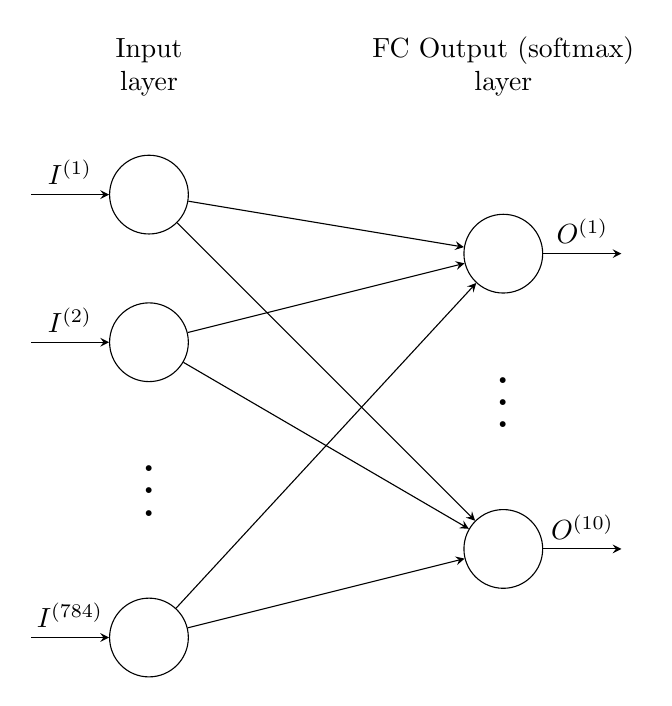
\begin{tikzpicture}[x=1.5cm, y=1.5cm, >=stealth]

\foreach \m/\l [count=\y] in {1,2,missing,3}
  \node [every neuron/.try, neuron \m/.try] (input-\m) at (1.5,2.5-\y*1.25) {};

\foreach \m [count=\y] in {1,missing,2}
  \node [every neuron/.try, neuron \m/.try ] (conv1-\m) at (4.5,2-\y*1.25) {};

\foreach \l [count=\i] in {1,2,784}
  \draw [<-] (input-\i) -- ++(-1,0)
    node [above, midway] {$I^{\left(\l\right)}$};

\foreach \l [count=\i] in {1,10}
  \draw [->] (conv1-\i) -- ++(1,0)
    node [above, midway] {$O^{\left(\l\right)}$};

\foreach \i in {1,...,3}
  \foreach \j in {1,...,2}
    \draw [->] (input-\i) -- (conv1-\j);

\foreach \l [count=\x from 0] in {Input, FC Output (softmax)}
  \node [align=center, above] at (\x*3+1.5,2) {\l \\ layer};
\end{tikzpicture}
\caption{The Fully Connected Neural Network}
\end{figure}
where the input vector is the vector-form (size: $1\times784$) of the input image (size: $28\times28$), and the output vector is the prediction $10$-D vector. The edges between input layer and the output layer are the transition weight matrix $\mathbf{W}$ (size: $784\times10$). The mathematical model of the structure would be
$$\hat{\mathbf{Y}} = \boldsymbol{\sigma}\left(\mathbf{X}\mathbf{W} + \begin{bmatrix}\mathbf{b} \\
\vdots \\
\mathbf{b}
\end{bmatrix}\right)\text{,}$$
and we take the cross-entropy loss function
$$L\left(\mathbf{Y}, \hat{\mathbf{Y}}\right) = -\frac1N\sum\limits_{n \in N}\sum\limits_{i = 1}^{10}Y_{n,i}\log\hat{Y}_{n,i}\text{.}$$
Applying the backpropagation \cite{rumelhart1988learning} based on chain rules we obtained
$$\frac{\partial L}{\partial\mathbf{W}} = \frac{\partial\hat{\mathbf{Y}}}{\partial \mathbf{W}}\frac{\partial L}{\partial\hat{\mathbf{Y}}} = \mathbf{X}^{\intercal}\left(\hat{\mathbf{Y}} - \mathbf{Y}\right)\text{,}$$
and for the bias term
$$\frac{\partial L}{\partial\mathbf{b}} = \sum\limits_{i \in N}\left(\hat{\mathbf{Y}} - \mathbf{Y}\right)_i$$
where $\left(\hat{\mathbf{Y}} - \mathbf{Y}\right)_i$ is the $i$-th row of $\hat{\mathbf{Y}} - \mathbf{Y}$.\par
Therefore each training step could be presented as follows
$$\mathbf{W}_{\text{new}} = \mathbf{W}_{\text{prev}} - \eta\frac{\partial L\left(\mathbf{Y}, \hat{\mathbf{Y}}\right)}{\partial\mathbf{W}},\, \mathbf{b}_{\text{new}} = \mathbf{b}_{\text{prev}} - \eta\frac{\partial L\left(\mathbf{Y}, \hat{\mathbf{Y}}\right)}{\partial\mathbf{b}}$$
where $\eta$ is the learning rate.
\subsection{Implementation by \texttt{numpy}}
Implementing the model by \texttt{numpy}, and setting the max training steps $10000$, batch size $100$, and learning rate $10^{-4}$, we have the iteration running result as the following picture
\begin{figure}[H]
\centering
\begin{minipage}[b]{0.45\textwidth}
\centering
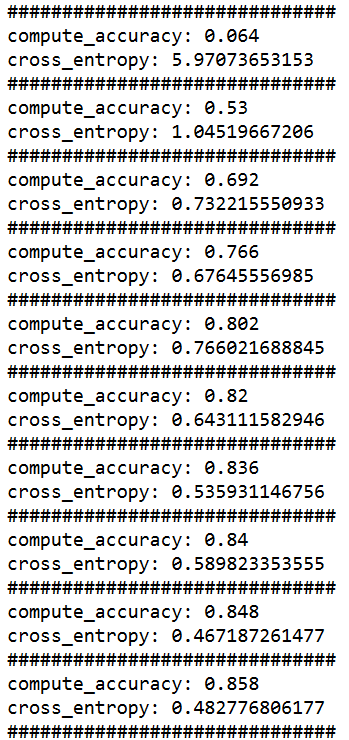
\includegraphics[scale=.95]{fig1.png}
\label{fig1}
\end{minipage}
\
\begin{minipage}[b]{0.45\textwidth}
\centering
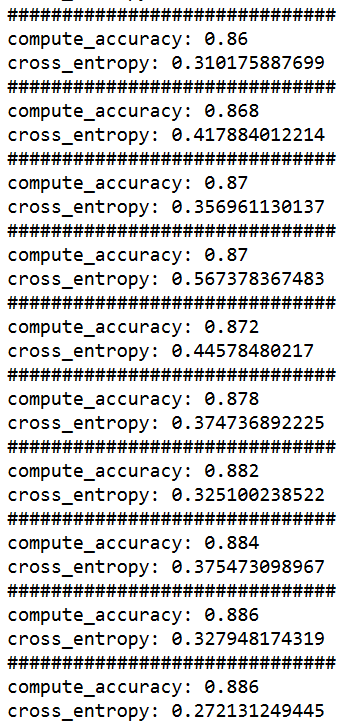
\includegraphics[scale=.95]{fig2.png}
\label{fig2}
\end{minipage}
\caption{The Iteration Result by \texttt{numpy}}
\end{figure}
and we have the accuracy plot and the loss plot against epochs for training and testing
\begin{figure}[H]
\centering
\begin{minipage}[b]{0.45\textwidth}
\centering
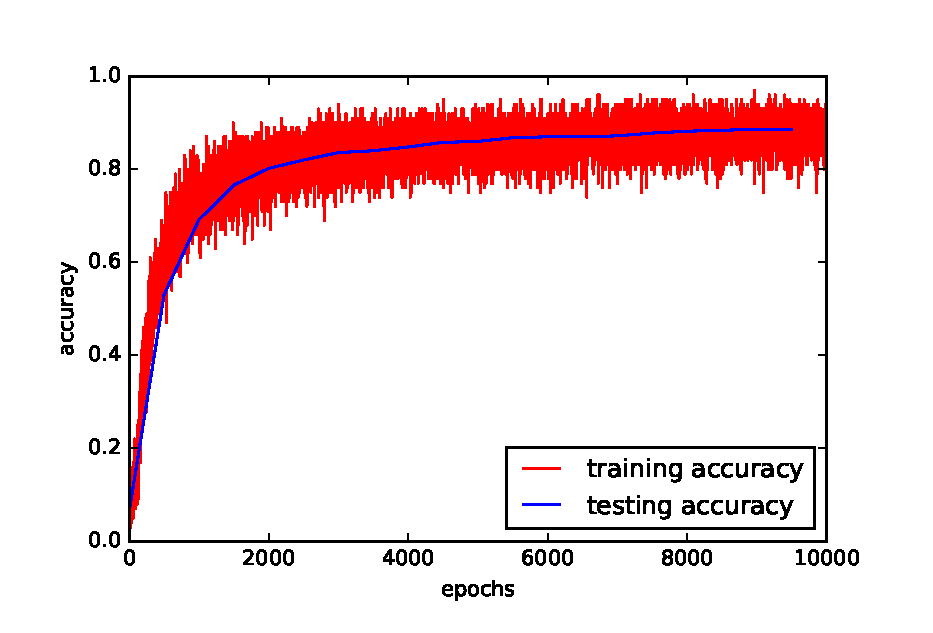
\includegraphics[scale=.5]{plot1.eps}
\caption{The Accuracy Plot against Epochs}
\label{plot1}
\end{minipage}
\
\begin{minipage}[b]{0.45\textwidth}
\centering
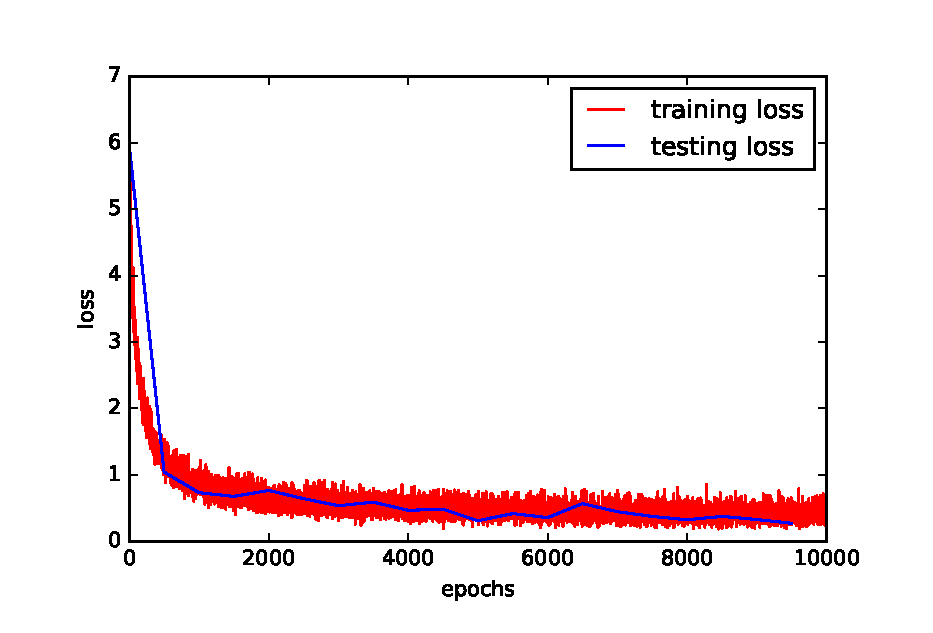
\includegraphics[scale=.5]{plot2.eps}
\caption{The Loss Plot against Epochs}
\label{plot2}
\end{minipage}
\end{figure}
As we observe from the iteration results and the plots, the accuracies and the losses of both training and testing show a sharp increasing and decreasing trend respectively in the prophase of the training process (the number of epochs is less than around $1500$), after which the trends of both slow down. For the training accuracy and loss, they show sharp oscillations during the whole process. The final testing accuracy is $0.886$, of which the cross entropy loss is $0.272131$.
\subsection{Implementation by \texttt{tensorflow}}
We take the softmax cross entropy as the loss function (the same as the loss function in the \texttt{numpy} model), setting the max epochs to $3000$, the learning rate to $0.1$, and the batch size to $100$, using the adam optimizer, we have the running result as the picture shows below
\begin{figure}[H]
\centering
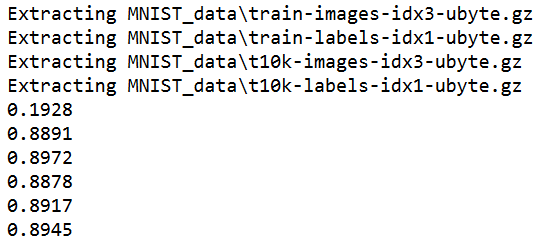
\includegraphics[scale=0.9]{fig3.png}
\caption{The Iteration Result by \texttt{tensorflow}}
\label{fig3}
\end{figure}
and we have the accuracy plot and the loss plot against epochs for training and testing
\begin{figure}[H]
\centering
\begin{minipage}[b]{0.45\textwidth}
\centering
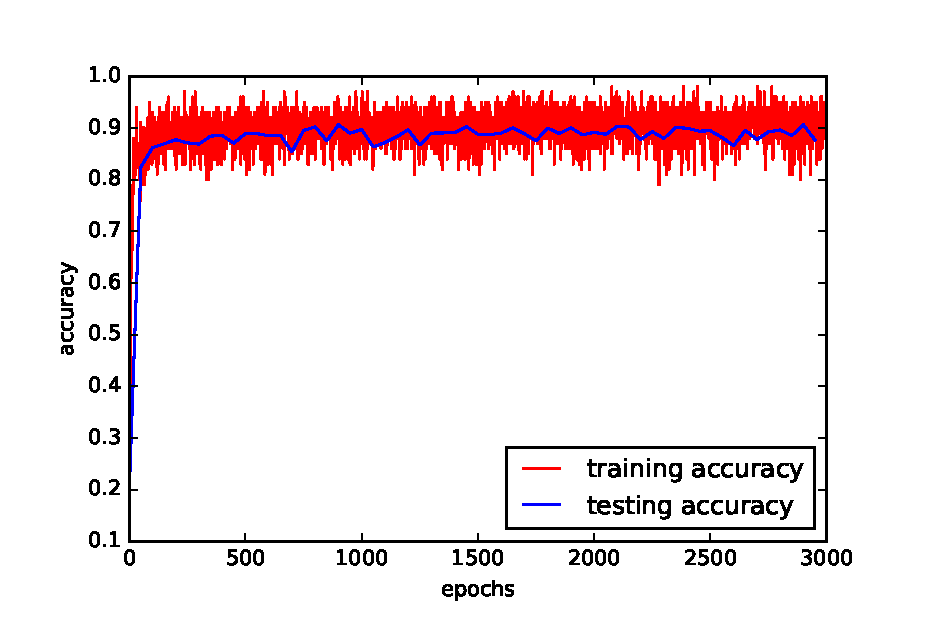
\includegraphics[scale=.45]{plot3.eps}
\caption{The Accuracy Plot against Epochs}
\label{plot3}
\end{minipage}
\
\begin{minipage}[b]{0.45\textwidth}
\centering
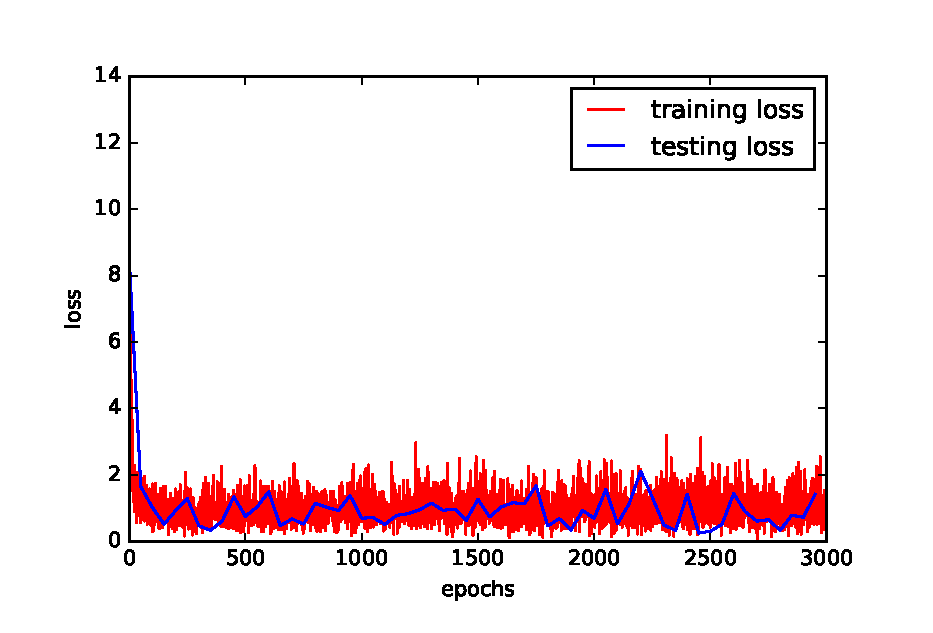
\includegraphics[scale=.45]{plot4.eps}
\caption{The Loss Plot against Epochs}
\label{plot4}
\end{minipage}
\end{figure}
As we observe from the running result picture and the plots, the convergence speed is much faster than the \texttt{numpy} based model (probably because the adam optimizer is much more efficient than normal gradient descent method). This model shows a steady convergence state as the number of epochs reaches $100$. The final testing accuracy is $0.8945$, of which the cross entropy loss is $0.30369076$.\par
As we observe from the result above, this model's capability has reached its limit as those two methods above showed a convergent state without overfitting. In order to optimize the model, we decide to adjust the structure, inserting a hidden layer (with $1024$ neurons) between the appeared two layers
\begin{figure}[H]
\centering
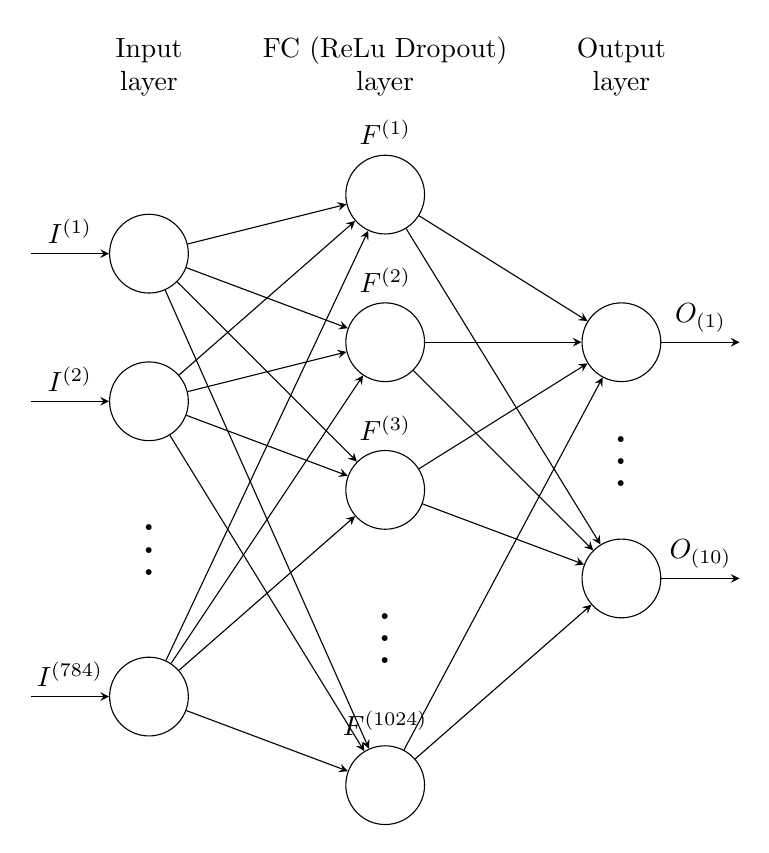
\begin{tikzpicture}[x=1.5cm, y=1.5cm, >=stealth]

\foreach \m [count=\y] in {1,2,missing,3}
  \node [every neuron/.try, neuron \m/.try ] (input-\m) at (1,2-\y*1.25) {};

\foreach \m [count=\y] in {1,2,3,missing,4}
  \node [every neuron/.try, neuron \m/.try ] (fc-\m) at (3,2.5-\y*1.25) {};

\foreach \m [count=\y] in {1,missing,2}
  \node [every neuron/.try, neuron \m/.try ] (output-\m) at (5,1-\y) {};

\foreach \l [count=\i] in {1,2,3,1024}
  \node [above] at (fc-\i.north) {$F^{\left(\l\right)}$};

\foreach \l [count=\i] in {1,2,784}
  \draw [<-] (input-\i) -- ++(-1,0)
    node [above, midway] {$I^{\left(\l\right)}$};

\foreach \l [count=\i] in {1,10}
  \draw [->] (output-\i) -- ++(1,0)
    node [above, midway] {$O_{\left(\l\right)}$};

\foreach \i in {1,...,3}
  \foreach \j in {1,...,4}
    \draw [->] (input-\i) -- (fc-\j);

\foreach \i in {1,...,4}
  \foreach \j in {1,...,2}
    \draw [->] (fc-\i) -- (output-\j);

\foreach \l [count=\x from 0] in {Input, FC (ReLu Dropout), Output}
  \node [align=center, above] at (\x*2+1,2) {\l \\ layer};
\end{tikzpicture}
\end{figure}
where the hidden layer has activation function \texttt{ReLu} and a dropout layer with keep probability $0.9$. The training result is better than the previous model. And the final testing accuracy will reach around $0.92$, which is a little bit greater than the model without a hidden layer. The running result is shown as follows
\begin{figure}[H]
\centering
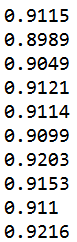
\includegraphics[scale=0.9]{fig4.png}
\caption{The Iteration Result with a hidden layer by \texttt{tensorflow}}
\label{fig3}
\end{figure}
\section{Conclusion}
Both \texttt{numpy} and \texttt{tensorflow} based models show convergent trends (accuracy around $0.9$) with the training processes pass, and they are both not overfitting. The optimizer of the loss function is the key to the efficiency of the training process.\par
By adjusting the structure of the network, we can also learn that the complexity of a model is a key point to improve the fitting performance. Sometimes, a network with more complex structure has a stronger capability to fit large-scale data.
\bibliographystyle{plain}
\bibliography{ref}
\end{document}